% Created 2011-07-17 Sun 09:10
\documentclass{beamer}
\usepackage[utf8]{inputenc}
\usepackage[T1]{fontenc}
\usepackage{fixltx2e}
\usepackage{graphicx}
\usepackage{longtable}
\usepackage{float}
\usepackage{wrapfig}
\usepackage{soul}
\usepackage{textcomp}
\usepackage{marvosym}
\usepackage[integrals]{wasysym}
\usepackage{latexsym}
\usepackage{amssymb}
\usepackage{hyperref}
\tolerance=1000
\usepackage{amsmath}
\usepackage{blkarray}

\usetheme[secheader]{Boadilla}
\usepackage[english]{babel}
\setbeamercolor{title}{fg=black,bg=black!10!brown!50}
\setbeamercolor{block body}{fg=black,bg=black!10!brown!30}
\setbeamercolor{block title}{fg=black,bg=black!30!brown!40}
\setbeamercolor{frametitle}{fg=black,bg=black!30!brown!50}
\beamersetaveragebackground{brown!50!black!20}
\setbeamercolor{author in head/foot}{fg=black,bg=black!30!brown!50}
\setbeamercolor{title in head/foot}{fg=black,bg=black!20!brown!50}
\setbeamercolor{date in head/foot}{fg=black,bg=black!10!brown!50}
\setbeamercolor{section in head/foot}{fg=black,bg=black!30!brown!30}
\setbeamercolor{subsection in head/foot}{fg=black,bg=black!20!brown!30}
\usepackage{animate} %need the animate.sty file 
\usepackage{color}
\usepackage{pgf}
\usepackage{pgfcore}
\usepackage{pgfbaseimage}
\usepackage{pgfbaselayers}
\usepackage{pgfbasepatterns}
\usepackage{pgfbaseplot}
\usepackage{pgfbaseshapes}
\usepackage{pgfbasesnakes}
\usepackage{tikz} 

\tikzset{normal/.style={ 
% The shape: 
rectangle,minimum size=6mm,rounded corners=3mm, 
% The rest 
very thick,draw=black!50, 
top color=white,bottom color=black!20, 
font=\ttfamily}}
\tikzset{arduino/.style={ 
% The shape: 
rectangle, 
% The size: 
minimum size=6mm, 
% The border: 
very thick, 
draw=blue!50!black!50, % 50% red and 50% black, 
% and that mixed with 50% white 
% The filling: 
top color=white, % a shading that is white at the top... 
bottom color=blue!50!black!20, % and something else at the bottom 
% Font 
font=\itshape 
}}
\tikzset{enceinte/.style={ 
% The shape: 
rectangle, 
% The size: 
minimum size=6mm, 
% The border: 
very thick, 
draw=yellow!90!black!50, % 50% red and 50% black, 
% and that mixed with 50% white 
% The filling: 
top color=white, % a shading that is white at the top... 
bottom color=yellow!90!black!20, % and something else at the bottom 
% Font 
font=\itshape 
}}

\tikzset{ordi/.style={ 
% The shape: 
rectangle, 
% The size: 
minimum size=6mm, 
% The border: 
very thick, 
draw=green!90!black!50, % 50% red and 50% black, 
% and that mixed with 50% white 
% The filling: 
top color=white, % a shading that is white at the top... 
bottom color=green!90!black!20, % and something else at the bottom 
% Font 
font=\itshape 
}}

\usetikzlibrary{decorations.pathmorphing,shapes.misc}
\providecommand{\alert}[1]{\textbf{#1}}

\date{\today}

\title[Reducing dimensionality]{Reducing the Dimensionality of the Reward Space in the Inverse Reinforcement Learning Problem}
\author[Olivier Pietquin]{{Edouard Klein}$^{\dag\ddag}$, Matthieu Geist$^\dag$ and \underline{Olivier Pietquin}$^\dag$\\\texttt{firstname.lastname@supelec.fr}}\institute[Supélec]{$\dag$Supélec UMI 2958 (GeorgiaTech - CNRS), France\\$\ddag$Equipe ABC UMR 7503 (LORIA-CNRS), France}
\begin{document}

\maketitle
\tikzstyle{state}=[circle,
thick,
minimum size=1.0cm,
draw=blue!80,
fill=blue!20]
\tikzstyle{action}=[rectangle,thick,
minimum size=1.0cm,
draw=orange!80,
fill=orange!20]
\tikzstyle{element}=[rectangle,
thick,
minimum size=1.0cm,
draw=blue!80,
fill=blue!20]
\tikzstyle{action}=[rectangle,thick,
minimum size=1.0cm,
draw=orange!80,
fill=orange!20]
\section{Non-technical Abstract}
\label{sec-1}
\subsection{Context}
\label{sec-1_1}
\begin{frame}
\frametitle{Reinforcement Learning}
\label{sec-1_1_1}
\begin{columns}
\begin{column}{0.4\textwidth}
%% Toto
\label{sec-1_1_1_1}

     
\includegraphics[width=10em]{ML.png}
\end{column}
\begin{column}{0.4\textwidth}
\begin{block}{Notions}
\label{sec-1_1_1_2}


\begin{itemize}
\item Agent
\item Task
\item Environment
\end{itemize}
\end{block}
\end{column}
\end{columns}
\end{frame}
\begin{frame}
\frametitle{Imitation: Expert}
\label{sec-1_1_2}

     \animategraphics[autoplay,loop,height=5cm]{1}{Expert00}{1}{9} 
\end{frame}
\begin{frame}
\frametitle{Imitation: Generalization}
\label{sec-1_1_3}
\begin{columns}
\begin{column}{.4\textwidth}
%% Null
\label{sec-1_1_3_1}

      \animategraphics[autoplay,loop,height=5cm]{1}{Agent}{001}{014} 
\end{column}
\begin{column}{.4\textwidth}
\begin{block}{Apprenticeship learning}
\label{sec-1_1_3_2}

     Reward inference
\end{block}
\end{column}
\end{columns}
\end{frame}
\subsection{Contribution}
\label{sec-1_2}
\begin{frame}
\frametitle{Contribution}
\label{sec-1_2_1}

\begin{block}<1->{Proposition}
  The dimension of the reward space to be searched can be reduced by two for all MDPs.
\end{block}
\begin{block}<2>{Algorithm}
  Similar to the search for basic feasible solutions in the simplex algorithm. Experimentally promising, needs more theoretical work.
\end{block}
\end{frame}
\section{IRL}
\label{sec-2}
\subsection{RL}
\label{sec-2_1}
\begin{frame}
\frametitle{Quick definitions}
\label{sec-2_1_1}

       \begin{columns}
    \begin{column}{4cm}
      \begin{block}{}
        \begin{overlayarea}{\textwidth}{4.4cm}
          \only<1>{\begin{tikzpicture}
  \node[state] (st) at (0,0) {$s_t$};
  \node at (0,1.5) {};
\end{tikzpicture}
}
          \only<2>{\begin{tikzpicture}
  \node[state] (st) at (0,0) {$s_t$};
  \node[action] (st) at (1.5,-2) {$a_{t}$};
  \node at (0,1.5) {};
\end{tikzpicture}
}
          \only<3>{\begin{tikzpicture}
  \node[state] (st) at (0,0) {$s_t$};
  \node[action] (at) at (1.5,-2) {$a_{t}$};
  \node[state] (stpu) at (3,0) {$s_{t+1}$};
  \draw[->,thick] (at) --  (stpu);
  \draw[->,thick] (st) -- node[below] {$p(s_{t+1}|s_t,a_t)$}(stpu);
  \node at (0,1.5) {};
\end{tikzpicture}
}
          \only<4->{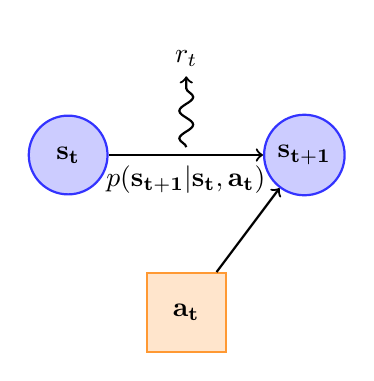
\begin{tikzpicture}
\tikzstyle{state}=[circle,
thick,
minimum size=1.0cm,
draw=blue!80,
fill=blue!20]
\tikzstyle{action}=[rectangle,thick,
minimum size=1.0cm,
draw=orange!80,
fill=orange!20]

  \node[state] (st) at (0,0) {$\mathbf{s_t}$};
  \node[action] (at) at (1.5,-2) {$\mathbf{a_{t}}$};
  \node[state] (stpu) at (3,0) {$\mathbf{s_{t+1}}$};
  \draw[->,thick] (at) --  (stpu);
  \draw[->,thick] (st) -- node[below] {$p(\mathbf{s_{t+1}}|\mathbf{s_t},\mathbf{a_t})$}(stpu);
  \draw[->,thick,decorate,decoration={snake}] (1.5,0.1) -- (1.5,1);
  \node[anchor=south] at (1.5,1.0) {$r_t$};
  \node at (0,1.5) {};
\end{tikzpicture}
}
        \end{overlayarea}
      \end{block}
    \end{column}
    \begin{column}{4cm}
      \begin{block}{Notions}
        \begin{itemize}
          \item<1-> State $s_t\in S$
          \item<2-> Action $a_t \in A$
          \item<3-> Reward $r_t \in \mathbb{R}$
          \item<4-> Transition $(s_t,a_t,s_{t+1},r_t)\in S\times A\times S\times\mathbb{R}$
        \end{itemize}
      \end{block}
      \begin{block}<1->{Markovian criterion}
        Past states are irrelevant
      \end{block}
    \end{column}
  \end{columns}
  \begin{alertblock}<5>{Policy}
    $\pi: S\rightarrow A$
  \end{alertblock}
\end{frame}
\begin{frame}
\frametitle{RL problem and solution}
\label{sec-2_1_2}
\begin{block}<1->{Value function}
\label{sec-2_1_2_1}

     \begin{equation}
     \label{eqn:V}
     V^\pi(s_t) = E\left[\left.\sum\limits_{i}\gamma^i r_{t+i}\right|\pi\right]
     \end{equation}
\end{block}
\begin{block}<2->{Goal}
\label{sec-2_1_2_2}

     Optimal policy $\pi^* = \arg\max\limits_\pi V^\pi$
\end{block}
\begin{block}<3->{Bellman equation (matrix form)}
\label{sec-2_1_2_3}

     $V^\pi = R + \gamma P^\pi V^\pi$
\end{block}
\end{frame}
\subsection{IRL}
\label{sec-2_2}
\begin{frame}
\frametitle{IRL problem and solutions}
\label{sec-2_2_1}
\begin{block}<1->{Goal}
\label{sec-2_2_1_1}

     Finding the reward $R$ so that the observed behavior is optimal
\end{block}
\begin{alertblock}<2->{Ill-posed}
\label{sec-2_2_1_2}

     The null reward $\forall s, R(s) = 0$ is a solution
\end{alertblock}
\begin{block}<3->{Linear constraints}
\label{sec-2_2_1_3}

\begin{equation}
  \label{ng2000algorithms.eqn}
  (P_\pi-P_{a})(I-\gamma P_\pi)^{-1}R\succeq 0
\end{equation}

\end{block}
\end{frame}
\section{Contribution}
\label{sec-3}
\subsection{Proposition}
\label{sec-3_1}
\begin{frame}
\frametitle{Dimensionality reduction}
\begin{block}<1->{Definition}
  $\Pi^*(R) = \left\{\pi^* | \forall \pi, V^{\pi^*}_R\succeq  V^{\pi}_R\right\}$
\end{block}
\begin{block}<2->{Definition : Equivalence}
  $\Pi^*(R_1) = \Pi^*(R_2) \Leftrightarrow R_1 \equiv R_2$
\end{block}
\begin{block}<3->{Lemmas}
$\exists \alpha > 0, R_2=\alpha R_1 \Rightarrow R_1\equiv R_2$\\
$\exists \lambda \in \mathbb{R}, R_2= R_1 + \lambda\mathbf{1} \Rightarrow R_1\equiv R_2$
\end{block}
\begin{alertblock}<4->{Proposition}
   $M = \{R|\mathbf{1}^TR =  0, ||R||_1 = 1\}$\\
   $\forall R \in \mathbb{R}^{|S|}\setminus \{ \lambda \mathbf{1}, \lambda \in \mathbb{R}\}, \exists R'\in M, R'\equiv R$.
\end{alertblock}
\end{frame}
\subsection{Algorithm}
\label{sec-3_2}
\begin{frame}
\frametitle{An algorithm making use of the new proposition}
\begin{columns}
\begin{column}{.45\textwidth}
\begin{block}<1->{}
  $(P_\pi-P_{a})(I-\gamma P_\pi)^{-1}R\succeq 0$\\
  $\mathbf{1}^TR =  0$\\
  $||R||_1 = 1$  
\end{block}
\begin{block}<2->{}
  \begin{eqnarray*}
  &C'R' \succeq 0 \\
  &\mathbf{1}'^TR'=0\\
  &||R||_1=1\\
  &R'\succeq 0\\
  \end{eqnarray*}
\end{block}
\end{column}
\begin{column}{.45\textwidth}
\begin{block}<3>{}
  \begin{eqnarray*}
  \label{LPStandardForm.eqn}
  \begin{blockarray}{(cc)}
  \begin{block*}{c|c}
  C'& -Id_m  \\
  \cline{1-2}
  \begin{block*}{c|c}
  \mathbf{1}'^T&0 \\
  \end{block*}
  \cline{1-2}
  \begin{block*}{c|c}
  \mathbf{1}^T\mathbf{1}^T&0 \\
  \end{block*}
  \end{block*}
  \end{blockarray} 
  \begin{blockarray}{(c)}
  \begin{block*}{c}
  R' \\
  \cline{1-1}
  \begin{block*}{c}
  S\\
  \end{block*}
  \end{block*}
  \end{blockarray}
  = 
  \begin{blockarray}{(c)}
  \begin{block*}{c}
  0 \\
  \vdots \\
  0 \\
  1\\
  \end{block*}
  \end{block*}
  \end{blockarray}\\
  \label{C1.eqn}
  R'\succeq 0\\
  \label{C2.eqn}
  S \succeq 0
  \end{eqnarray*}

\end{block}
\end{column}
\end{columns}
\end{frame}
\section{Experimental benchmark}
\subsection{GirdWorld}
\label{sec-4_3}
\begin{frame}
\frametitle{Settings}
\label{sec-4_3_1}
\begin{columns}
\begin{column}{0.4\textwidth}
%% Toto
\label{sec-4_3_1_1}


\includegraphics[width=10em]{Expert001.png}
\end{column}
\begin{column}{0.4\textwidth}
\begin{block}{Mathematically}
\label{sec-4_3_1_2}
\begin{itemize}
\item $A = \{$ Up, Down, Right, Left $\}$
\item $S = {cells}$
\item $\phi$: discrete features
\item Reward in the upper right corner
\end{itemize}
\end{block}
\end{column}
\end{columns}
\end{frame}
\subsection{Results}
\begin{frame}
\frametitle{Results}
\label{sec-4_3_1}
\begin{columns}
\begin{column}{0.4\textwidth}
%% Toto
\label{sec-4_3_1_1}
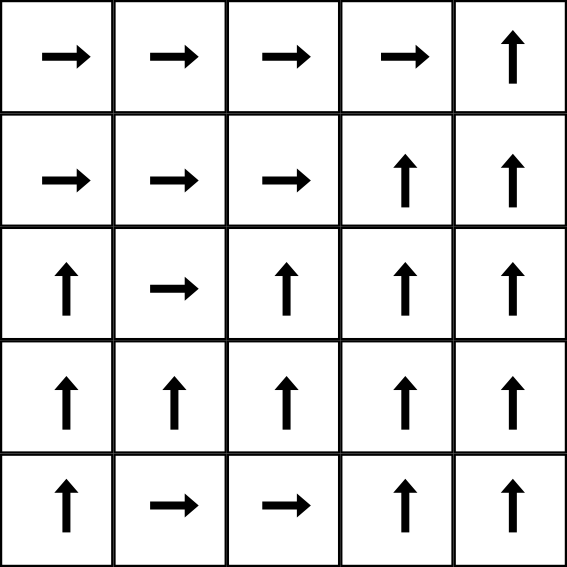
\includegraphics[width=10em]{Pi_E.png}
\end{column}
\begin{column}{0.4\textwidth}
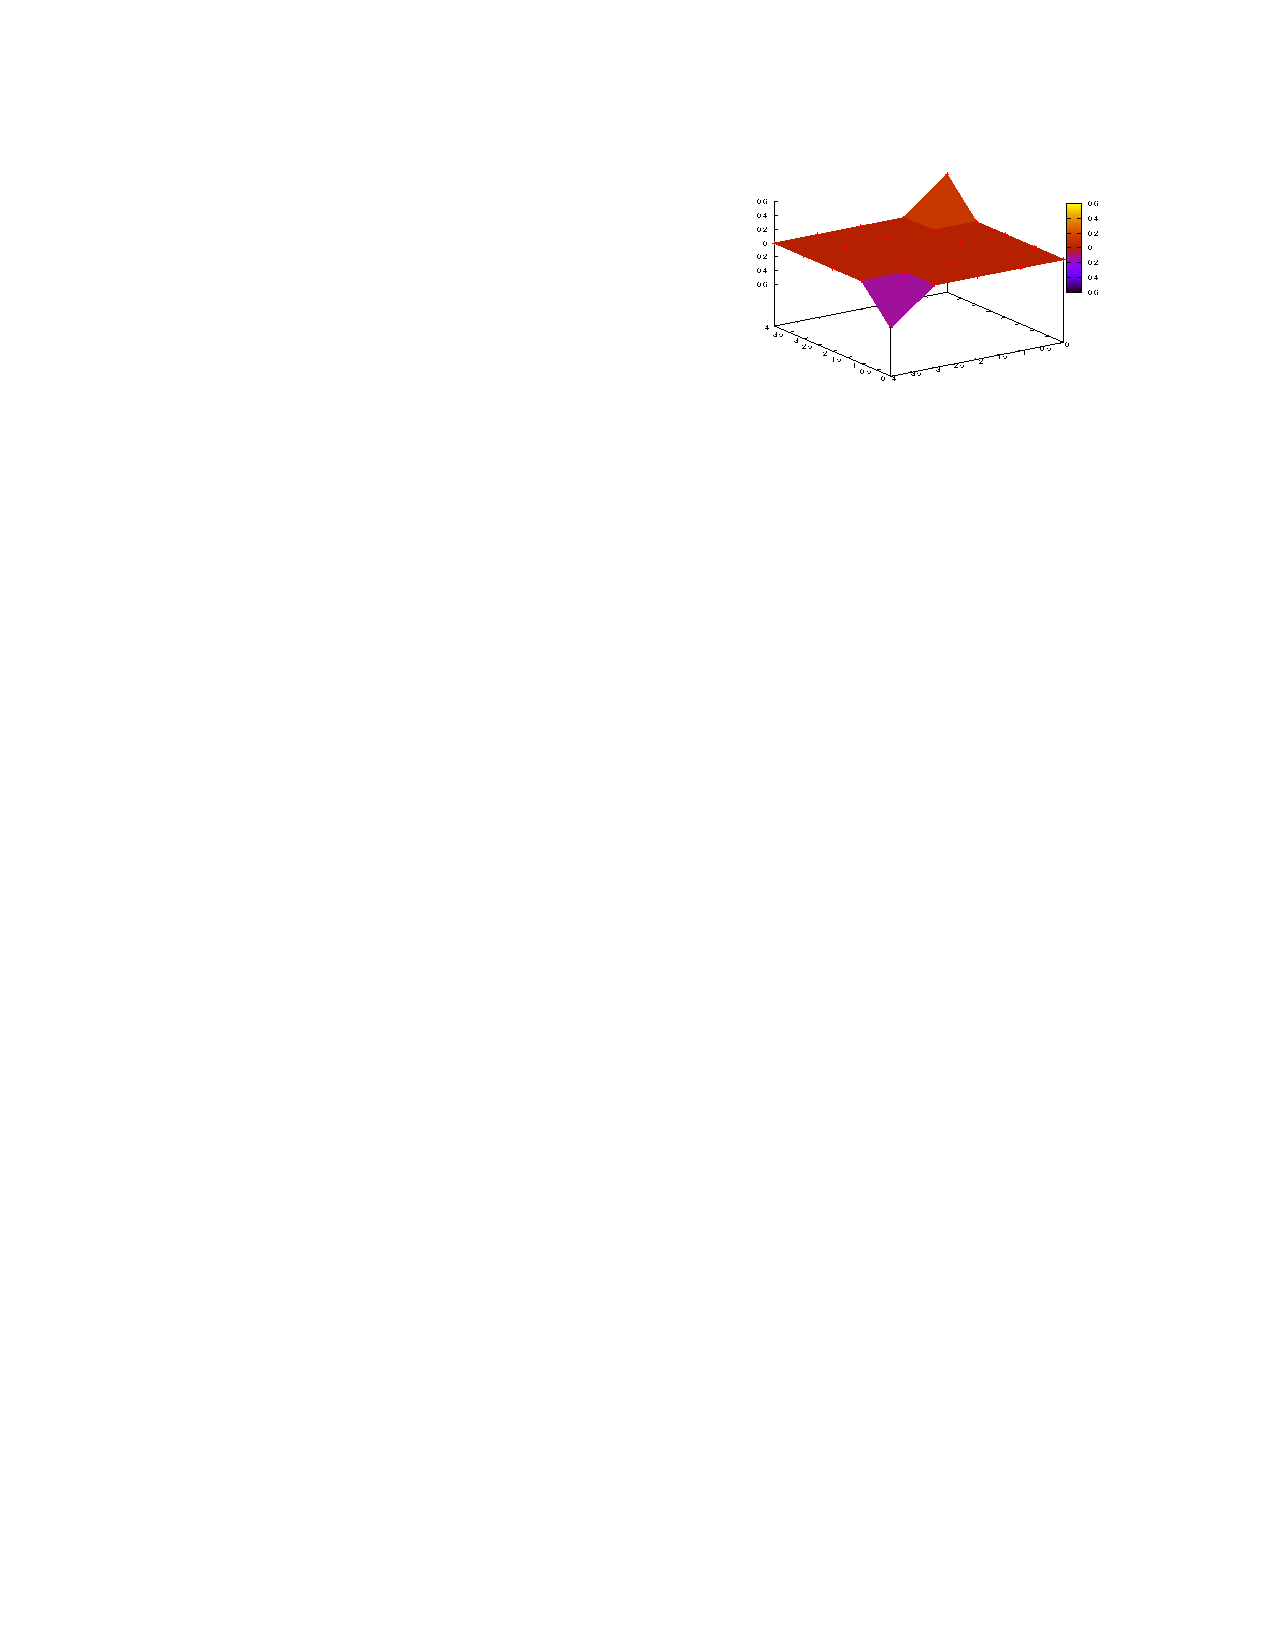
\includegraphics[width=\textwidth]{Results.pdf}
\end{column}
\end{columns}
\end{frame}
\section{Opening and future work}
\label{sec-5}
\subsection{Future work}
\label{sec-5_1}
\begin{frame}
\frametitle{Possible future work}
\label{sec-5_1_1}
\begin{itemize}
\item Characterization of MDPs our algorithm works on
\item State space transformation that guarantees that our algorithm works
\item Speeding up our algorithm
\item Sampling or approximation
\end{itemize} % ends low level
\end{frame}
\begin{frame}
\frametitle{Thank you\ldots{}}
\label{sec-5_1_2}

    \ldots{} for your attention
\end{frame}

\end{document}
